
\section{Introducción}
El diseño, desarrollo, fabricación, armado, simulación y lanzamiento de cohetes, no es una tarea
sencilla ni repetida en intervalos de cortos de tiempo, al contrario, suelen llevar décadas y una
fuerte inversión para que sean posibles estos logros. El diseño y auge de vehículos VTVL viene
a subsanar estos factores ya que una vez terminada la misión el vehículo se puede reutilizar,
con mínimas intervenciones, y estaría listo para una nueva misión, atacando estos dos puntos principales anteriormente mencionados, el tiempo y el costo. Esto es a diferencia del método convencional donde el vehículo, luego de completar la misión, pasa a formar parte de basura espacial o, en el mejor de los casos, es recuperado del mar como el caso del Space Shuttle. 

\medskip

Los vehículos VTVL son tan viejos como el primer alunizaje. Traen en si varias ventajas frente a otros vehículos voladores como la gran reducción de espacio necesario para despegar y aterrizar. Esto no es un detalle menor dado que la mayor parte de la superficie terrestre de la tierra no son pistas de aterrizaje si no más bien terreno formado naturalmente.

\medskip

Este documento propone el diseño, simulación, control y fabricación de un vehículo con capacidades VTVL siendo un prototipo de baja escala. 
Este prototipo serviría como punta pie inicial
para vehículos de escala mayor que puedan completar misiones espaciales. Existen varias ventajas de implementar este tipo de tecnología.

\medskip

A baja escala, un vehículo que despega y aterriza por su cuenta, teniendo la capacidad de
superar obstáculos que se presenten, puede ser de gran utilidad en ambientes hostiles para el
ser humano, que esto se logre de manera rápida y efectiva podría ser la diferencia entre el
éxito o no de la misión.
Como ser el transporte de insumos médicos en tiempo real desde que un paciente lo requiere,
en zonas de acceso limitado.

\medskip

Últimamente hay un interés nuevo en imágenes espaciales. El vehículo podría ser utilizado para fines de sistemas de monitoreo y análisis geoespacial mediante el uso de estas imágenes, como hacen las empresas \textit{Ceres Imaging} y \textit{Satellogic}. %de una situación en la que no se disponga del tiempo suficiente para el accionar convencional a bajas velocidades como ser un helicóptero o un dron.  

\medskip

El vehículo una vez desarrollado y funcionando, puede servir de plataforma para diversos
estudios de fenómenos de dinámica de fluidos, como ser, mediciones aerodinámicas,
investigación del \textit{fuel sloshing} en vehículos con tanques esbeltos.

\medskip


Los sistemas de vehículos orbitales tienen sistemas complejos que deben ser testeados en una primera etapa mediante algún ensayo controlado. El vehículo que se desarrolla en el presente documento podría ser usado para tales fines como una plataforma para pruebas como ser el despliegue de una nariz o etapa, comprobación de sensores y actuadores a gran velocidad y con empuje variable.



\subsection{Estudio - Agua como propelente}
Se estudió la posibilidad de propulsar el vehículo con agua a presión. La figura \ref{fig:bottlerocket} muestra los resultados de una simulación de un vehículo pequeño de aluminio con un tanque a presión lleno en parte de agua y aire a 200 bar. En el mejor de los casos se llegaba a un tiempo de vuelo cercano a los 4 segundos que no es suficiente para comprobar un sistema de control. 

Para optimizar este problema se modificaba

\begin{itemize}
    \item Diámetro de la tobera -- más empuje vs. menos tiempo de vuelo controlado
    \item Volumen de agua -- más tiempo de vuelo vs. mayor peso de vehículo
\end{itemize}


\begin{figure}[htb]
    \centering
    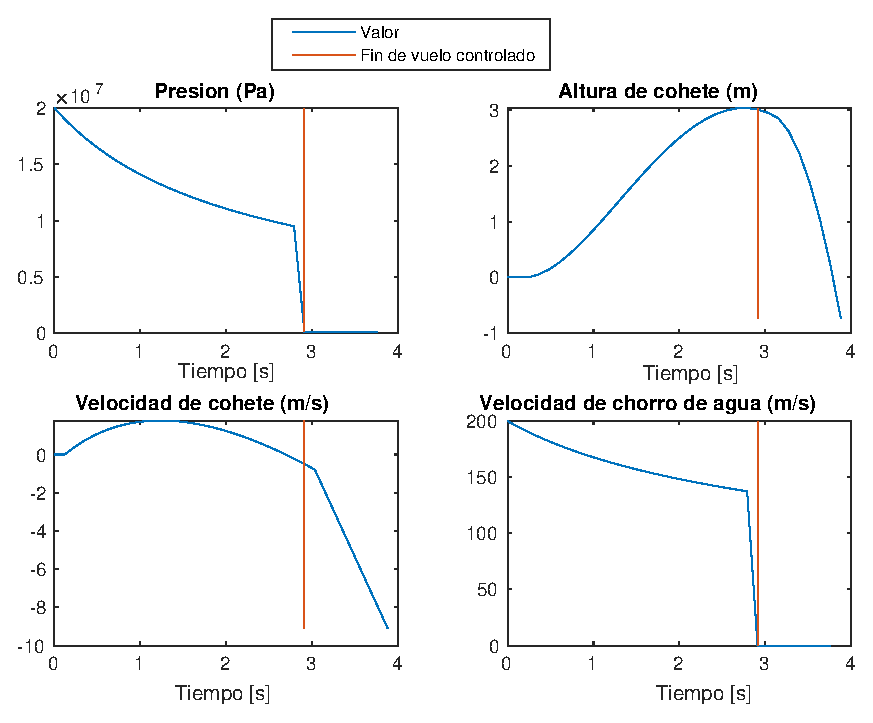
\includegraphics[width=0.8\linewidth]{fig/bottlerocket}
    \caption{Análisis preliminar para un vehículo propulsado por agua a presión. La presión es la del tanque (absoluta).}
    \label{fig:bottlerocket}
\end{figure}

\newpage


\subsection{Propulsión eléctrica}


\begin{figure}[htb]
    \centering
    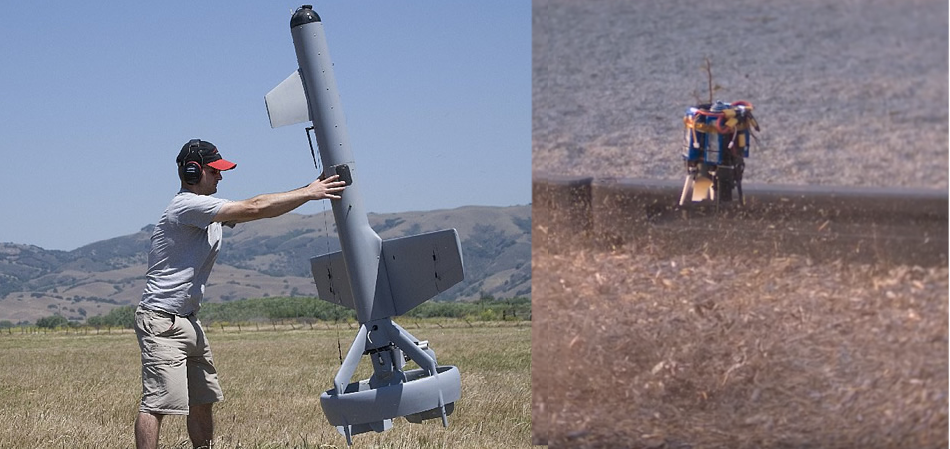
\includegraphics[width=0.8\linewidth]{fig/vbat_icarus.png}
    \caption{Dos vehículos VTVL eléctricos modernos. ``VBat'' (Izq.) y ``Ikarus'' (Der.).}
    \label{fig:vbat_icarus}
\end{figure}

%Estos vehículos suelen ser la primera de muchas etapas para el desarrollo de un vehículo que cumple con los requisitos de la misión final.
Para lograr estas tareas generalmente los vehículos VTVL de baja escala generalmente son propulsados por motores eléctricos. %También existen alternativas al método de propulsión que se consideraron pero dado el alcance de un proyecto de universidad se decidió por un diseño compuesto por elementos comercialmente disponibles.\footnote{\textit{Commercial off the shelf} (COTS)}

\medskip

Los vehículos VTVL eléctricos son propulsados por hélices en su mayoría y constan casi siempre de 3 o más propulsores en un arreglo simétrico y plano. Recientemente hay un interés por la construcción de vehículos de una sola hélice por la buena relación empuje--peso que tienen. Sin embargo, estos vehículos no vienen sin sus complicaciones: 

\begin{itemize}
    \item La rotación dada al aire por la hélice causa un momento en el eje de propulsión que es contrarrestado en vehículos multirrotores.
    \item Inclinar al rotor durante su funcionamiento causa una fuerza perpendicular a la dirección de inclinación conocido como el efecto giroscópico. 
\end{itemize}

El primer punto es mitigado fácilmente agregando álabes a la salida del chorro para enderezar el flujo y contrarrestar la rotación. El segundo punto solo se resuelve conociendo las ecuaciones de momento angular y controlando actuadores con un sistema de control a lazo cerrado. Los sistemas vistos en la figura \ref{fig:vbat_icarus} tienen la particularidad de poder ser representados con relativa facilidad usando un solo marco de referencia inercial para el cálculo de las ecuaciones de momento angular. 